\section{Theoretical Analysis}
\label{sec:analysis}

In this section, the circuit shown in Figure \ref{fig:t2} is analysed
theoretically, analysing the circuit for $t<0$, calculating the equivalent resistance, determining the natural and forced solutions and superimposing them to find the total solution.

\subsection{Nodal analysis}
For t$<$0,  $v_s(t)= V_s(t)$,  it is a DC circuit. We can determine the voltges in all nodes and currents in all branches using the nodal method.
Since this is a linear circuit,  we apply Ohm's Law,  $V_i= R_i * I$ and the Kirchoff Current Law (KCL),  $\sum I_i = 0$.

We get the following equation,  in matrix form:

\begin{equation}
\label{eq:matrixeq1}
\begin{bmatrix}
    -G_1 & G_1+G_2+G_3 & -G_2 & 0 & -G_3 & 0 & 0 & 0\\
    0 & -G_2-K_b & G_2 & 0 & K_b & 0 & 0 & 0\\
    0 & K_b & 0 & 0 & -G_5-K_b & G_5 & 0 & 0\\
    0 & 0 & 0 & -G_6 & 0 & 0 & G_6+G_7 & -G_7\\
    1 & 0 & 0 & -1 & 0 & 0 & 0 & 0\\
    0 & 0 & 0 & 0 & 0 & 0 & 0 & 1\\
    0 & 0 & 0 & -K_c*G_6 & 1 & 0 & K_c*G_6 & -1\\
    0 & -G_3 & 0 & -G_4 & G_4+G_3+G_5 & -G_5 & -G_7 & G_7
\end{bmatrix}
\cdot
\begin{bmatrix}
V_1 \\
V_2 \\
V_3 \\
V_4 \\
V_5 \\
V_6 \\
V_7 \\
V_8 
\end{bmatrix}
=
\begin{bmatrix}
0 \\
0 \\
0 \\
0\\
V_s\\
0 \\
0 \\
0
\end{bmatrix}
\end{equation}


This equation solved using octave yields the following results:

\begin{table}[H]
    \centering
    \begin{tabular}{|l|r|}
      \hline    
      {\bf Variable} & {\bf Value [A or V]} \\ \hline
      V_1 & 5.13612248730V \\ \hline 
V_2 & 4.88464690881V \\ \hline 
V_3 & 4.36195145882V \\ \hline 
V_4 & -0.00000000000V \\ \hline 
V_5 & 4.92000960269V \\ \hline 
V_6 & 5.69027079572V \\ \hline 
V_7 & -1.96654083449V \\ \hline 
V_8 & -2.94453891610V \\ \hline 
I_1 & 0.00024147744V \\ \hline 
I_2 & 0.00025321233V \\ \hline 
I_3 & -0.00001173489V \\ \hline 
I_4 & -0.00120106056V \\ \hline 
I_5 & -0.00025321233V \\ \hline 
I_6 & 0.00095958312V \\ \hline 
I_7 & 0.00095958312V \\ \hline 
I_S & -0.00024147744V \\ \hline 
I_b & -0.00025321233V \\ \hline 
I_c & -0.00000000000V \\ \hline 
I_e & -0.00095958312V \\ \hline 

    \end{tabular}
    \caption{Node Analysis Results for t$<$0}
    \label{tab:nodeanalysis}
  \end{table}
  
  
\subsection{Equivalent resistance}
Now,  we have to determine the equivalent resistance $R_eq$ as seen from the capacitor terminals. We take out all the independent voltage sources (make $V_s=0$) and replace the capacitor with a voltage source $Vx= V(6)-V(8)$. The values of$ V(6)$ and $V(8)$ were already obtained via nodal analysis in the previous subsection. To determine the current $I_x$ supplied by $V_x$ we run mesh analysis:


\begin{equation}\label{eq:matrixeq2}
\begin{bmatrix}
 R1+R3+R4 & -R3 & -R4 & 0\\
    -Kb*R3 &  Kb*R3-1 & 0 & 0\\ 
    -R4 & 0 & R4+R6+R7-Kd & 0\\
    0 & -R5 & Kd & R5 \\
\end{bmatrix}
\cdot
\begin{bmatrix}
I_A\\
I_B \\
I_C \\
I_D \\

    \end{bmatrix}
=
    \begin{bmatrix}
0 \\
0 \\
0 \\
V_x \\

    \end{bmatrix}
  \end{equation}

This yields the following results:

\begin{table}[H]
    \centering
    \begin{tabular}{|l|r|}
      \hline    
      {\bf Variable} & {\bf Value [A or V]} \\ \hline
      V_x & 8.63480971182V \\ \hline 
I_x & 0.00283856995V \\ \hline 
R_{equiv} & 3041.95770117000V \\ \hline 

    \end{tabular}
    \caption{Equivalent resistance}
    \label{tab:equivalentresistance}
  \end{table}
  
$I_D = I_x = $
    
$R_{eq} = \frac{V_x}{I_x}= $

This value is equal to $R_5$, which makes sense: since the current controled voltage source $V_d$ has null internal resistance,  all the current flows through mesh D (which only contains $V_d$ and$R_5$).


For the time constant:

$\tau = R_{eq} \cdot C = $


EXPLICAR PORQUE AQUI OU DPS NO FINAL DO REL
L
L
L
L



\subsection{Natural solution}

Using the capacitor voltage $V_x$ for $t<0$ as the initial condition, the natural solution of $v_{6n}(t)$ becomes:

\begin{equation}
\label{eq:solucaonatural}
v_{6n}(t)=V_x e^{\frac{-x}{1000R_5C}}
\end{equation}

This equation gives us the following plot in [0,20]ms:

  \begin{figure}[H] \centering
    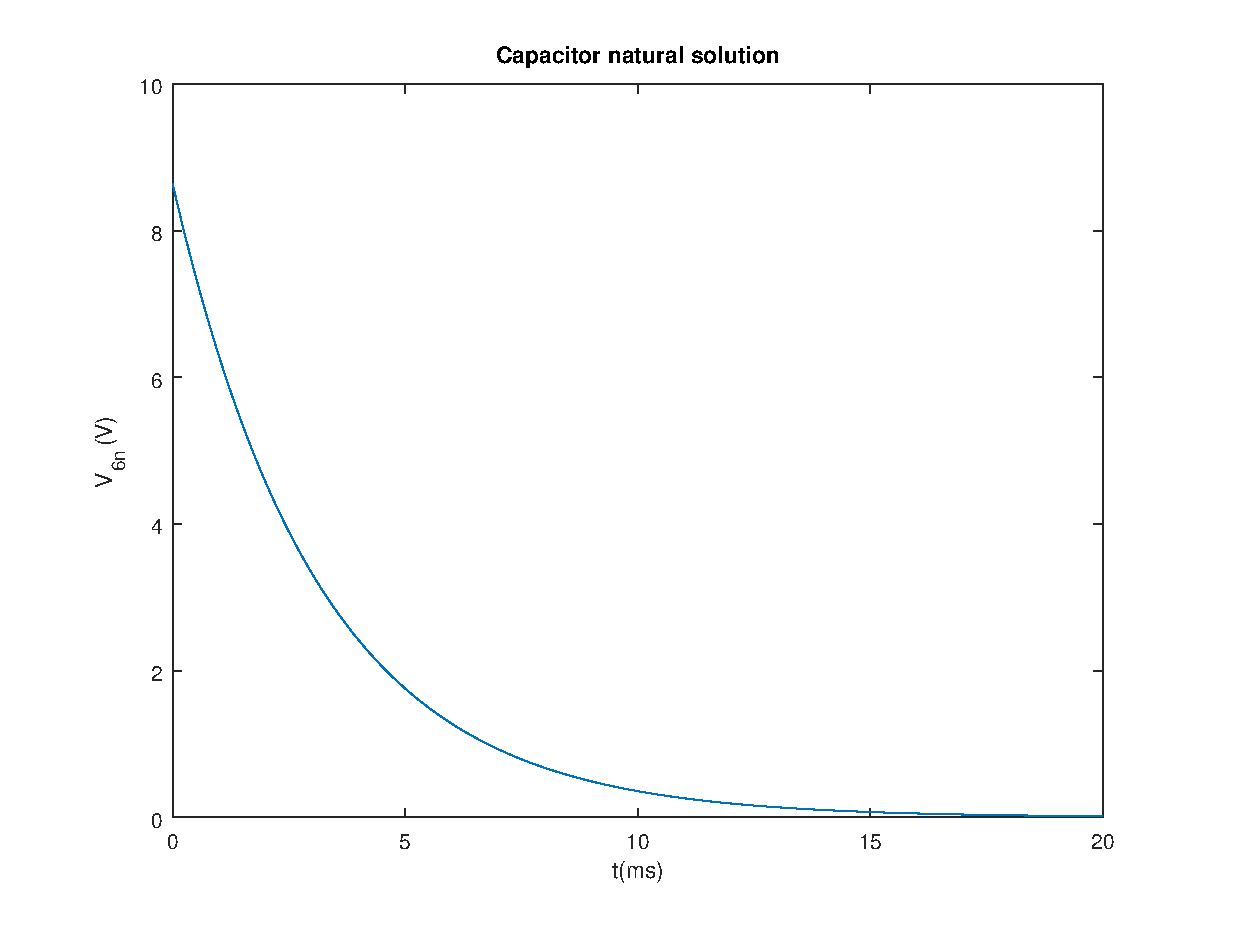
\includegraphics[width=1\linewidth]{natural.eps}
    \caption{Natural solution $v_{6n}(t)$}
    \label{fig:natural}
    \end{figure}



\subsection{Forced solution}

To determine the forced solution in the same interval [0, 20]ms we use a phasor voltage source $V_s$ and replace $C$ with its impedance $Z_c$.

We run nodal analysis to determine the phasor voltages in all nodes:

 $\omega=2*\pi*1000$
 
  \begin{equation}\label{eq:matrixeq3}
\begin{bmatrix}
-G1 & G1+G2+G3 & -G2 & 0 & -G3 & 0 & 0 & 0\\
0 & -G2-Kb & G2 & 0 & Kb & 0 & 0 & 0\\
0 & Kb & 0 & 0 & -G5-Kb & G5+(C*\omega*i) & 0 & -(C*\omega*i)\\
0 & 0 & 0 & -G6 & 0 & 0 & G6+G7 & -G7\\
1 & 0 & 0 & -1 & 0 & 0 & 0 & 0\\
0 & 0 & 0 & 1 & 0 & 0 & 0 & 0\\
0 & 0 & 0 & -Kd*G6 & 1 & 0 & Kd*G6 & -1\\
0 & -G3 & 0 & -G4 & G4+G3+G5 & -G5-(C*\omega*i) & -G7 & G7+(C*\omega*i)]
\end{bmatrix}
\cdot
\begin{bmatrix}
V_{1p} \\
V_{2p} \\
V_{3p} \\
V_{4p} \\
V_{5p} \\
V_{6p} \\
V_{7p} \\
V_{8p} 
    \end{bmatrix}
=
    \begin{bmatrix}
0 \\
0 \\
0 \\
0 \\
1 \\
0 \\
0 \\
0 
    \end{bmatrix}
  \end{equation}



Solving this system of equation in octave yiels the following results:

\begin{table}[H]
    \centering
    \begin{tabular}{|l|r|}
      \hline    
      {\bf Variable} & {\bf Value [A or V]} \\ \hline
      $\tilde{V}_1$ & $(0.00000000000+i\cdot1.00000000000)V$ \\ \hline 
$\tilde{V}_2$ & $(0.00000000000+i\cdot0.95103785412)V$ \\ \hline 
$\tilde{V}_3$ & $(0.00000000000+i\cdot0.84926936022)V$ \\ \hline 
$\tilde{V}_4$ & $(0.00000000000+i\cdot0.00000000000)V$ \\ \hline 
$\tilde{V}_5$ & $(0.00000000000+i\cdot0.95792294963)V$ \\ \hline 
$\tilde{V}_6$ & $(0.08501303490+i\cdot-0.56899006711)V$ \\ \hline 
$\tilde{V}_7$ & $(-0.00000000000+i\cdot-0.38288433334)V$ \\ \hline 
$\tilde{V}_8$ & $(-0.00000000000+i\cdot-0.57329997939)V$ \\ \hline
    \end{tabular}
    \caption{Phasor voltages}
    \label{tab:phasorvoltages}
  \end{table}
  
  

\subsection{Total solution}

Converting the phasors to real time functions for f=1KHz, we can then superimpose the natural and forced solutions:

$y_1=\Re(V_f(6)*e^(x*\omega*i/1000))+V_x*exp(-x/1000/R5/C)$

$y_2=\sin(\omega*x2/1000)$



  This plot in the interval [-5,20]ms:

  \begin{figure}[H] \centering
    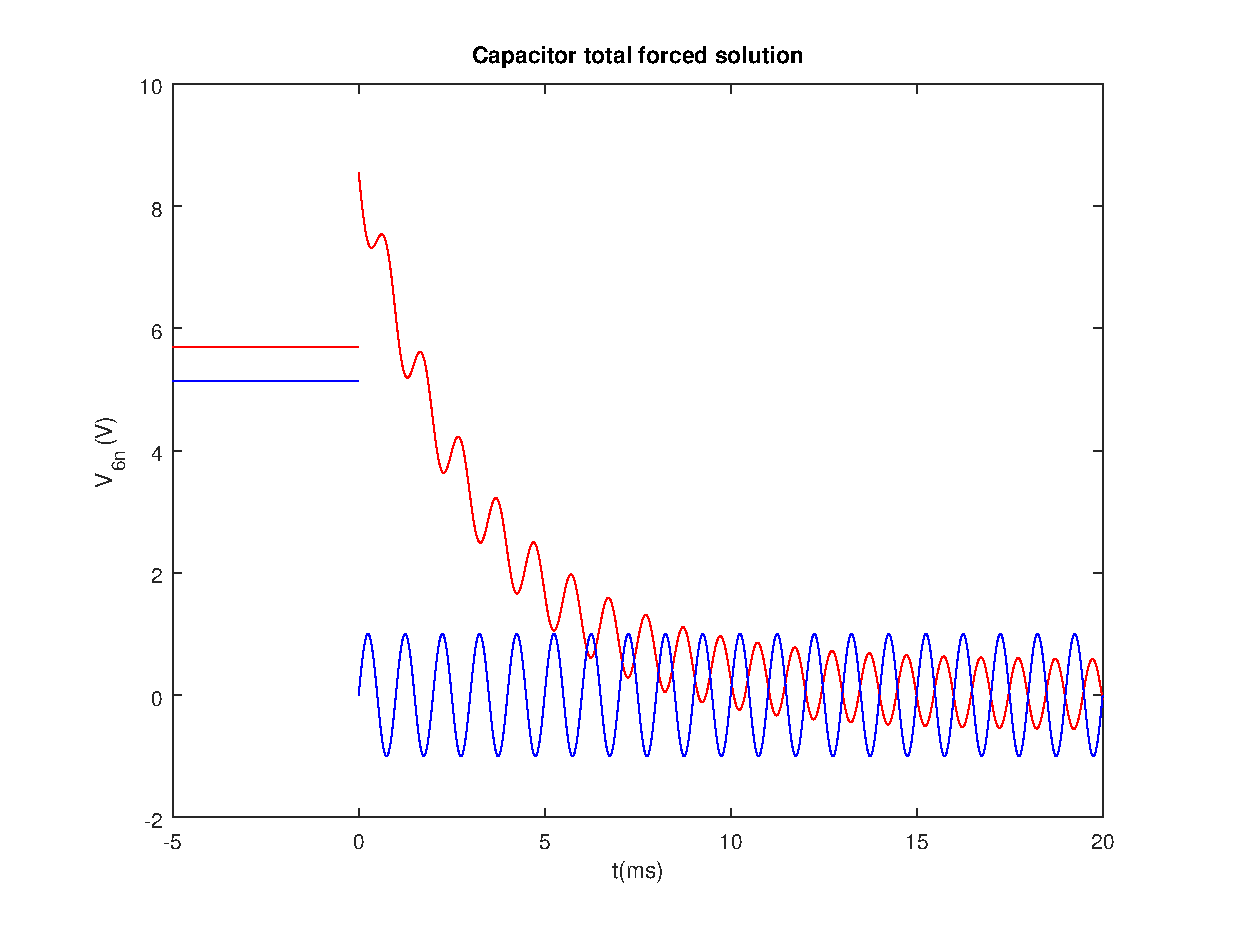
\includegraphics[width=1\linewidth]{forced.eps}
    \caption{Final total solution $v_{6}(t)$}
    \label{fig:total}
    \end{figure}
    
\subsection{Frequency responses}
      
  For the frequency responses, we get the following plot:
  
  
  EXPLICAR COMO E PORQUE DIFEREMM
  M
  M
